\section{Evaluation}
\label{sec:eval}

We extracted 50,000 questions from \emph{Stack Overflow} with titles, bodies and labels as our experiment dataset. To demonstrate our model's effectiveness on question texts, we excluded codes appeared in the body of questions and corresponding labels of programming languages. The frequency distribution of the dataset is indicated in Figure \ref{fig:labelperdoc} and \ref{fig:docperlabel}.

% \begin{figure}
% \centering
% \includegraphics[width=.7\columnwidth]{fig/freq_dist_1.eps}
% \caption{Number of documents that have $L$ labels}
% \label{fig:labelperdoc}
% \end{figure}

% \begin{figure}
% \centering
% \includegraphics[width=.7\columnwidth]{fig/freq_dist_2.eps}
% \caption{Number of labels that apear in $D$ documents}
% \label{fig:docperlabel}
% \end{figure}

\begin{figure*}
\centering
\subfigure[Number of documents that have $L$ labels]
    {\label{fig:labelperdoc}\includegraphics[width=.644\columnwidth]{fig/freq_dist_1.eps}}
\qquad
\subfigure[Number of labels that appear in $D$ documents]
    {\label{fig:docperlabel}\includegraphics[width=.644\columnwidth]{fig/freq_dist_2.eps}}
\qquad
\subfigure[Number of documents with different sizes]
    {\label{fig:docsizedist}\includegraphics[width=.644\columnwidth]{fig/freq_dist_3.eps}}
\qquad
\caption{\label{fig:s}Caption}
\end{figure*}

We compare the results with two other models, one is ``one-vs-all'' SVM classifiers without parameter tunning and Labeled LDA from Stanford Topic Modeling Toolbox. And the results are indicated in Table \ref{table:f1}.

\begin{table}[ht] 
\caption{$F_1$ scores for three models} % title of Table 
\centering % used for centering table 
{\small
    \begin{tabular}{c c c} 
    \hline
    SVM & L-LDA & \textbf{Q-LDA} \\ [0.5ex] % inserts table 
    \hline % inserts single horizontal line 
    0.540 & 0.613 & \textbf{0.620}\\ % inserting body of the table 
    \hline
    \end{tabular} 
}   
\label{table:f1} % is used to refer this table in the text 
\end{table}

Noted in our evaluation $F_1$ score is defined as 

\begin{equation}
F_1 = \frac{1}{K}\sum^K_{\lambda=1}{\frac
{2 \times \text{true positive}}
{2 \times \text{true positive} + \text{false negative} + \text{false positive}}}
\end{equation}

which is the macro averaged $F_1$ score for all labels.